\documentclass[conference]{IEEEtran}
\IEEEoverridecommandlockouts
% The preceding line is only needed to identify funding in the first footnote. If that is unneeded, please comment it out.
\usepackage{cite}
\usepackage{amsmath,amssymb,amsfonts}
\usepackage{graphicx}
\usepackage{textcomp}
\usepackage{xcolor}
\usepackage{siunitx}

\graphicspath{{./images}}


\def\BibTeX{{\rm B\kern-.05em{\sc i\kern-.025em b}\kern-.08em
    T\kern-.1667em\lower.7ex\hbox{E}\kern-.125emX}}
\begin{document}


\title{Automatické řízení - semestrální úloha}

\author{\IEEEauthorblockN{Vojtěch Michal}
michavo3@fel.cvut.cz}

\maketitle

\begin{abstract}
Report z modelování, analýzy a návrhu řízení pro dvoukolový segway postavený s vývojovou sadou LEGO Mindstorms.
Cílem práce je stabilizace segwaye v nestabilním svislém ekvilibriu a pohyb po rovné čáře.
\end{abstract}

\begin{IEEEkeywords}
    identifikace, linearizace, stabilizace, řízení, LEGO segway
\end{IEEEkeywords}

\section{Úvod}
\label{sec:uvod}
Segway je dvoukolové vozítko. Protože je těžiště umístěno nad osou otáčení, je nezbytné jej ve svislém nestabilním
ekvilibriu aktivně udržovat pomocí řízení. Cílem úlohy je analyzovat model segwaye a navrhnout pro něj řízení. 

\begin{figure}[htbp]
    \centerline{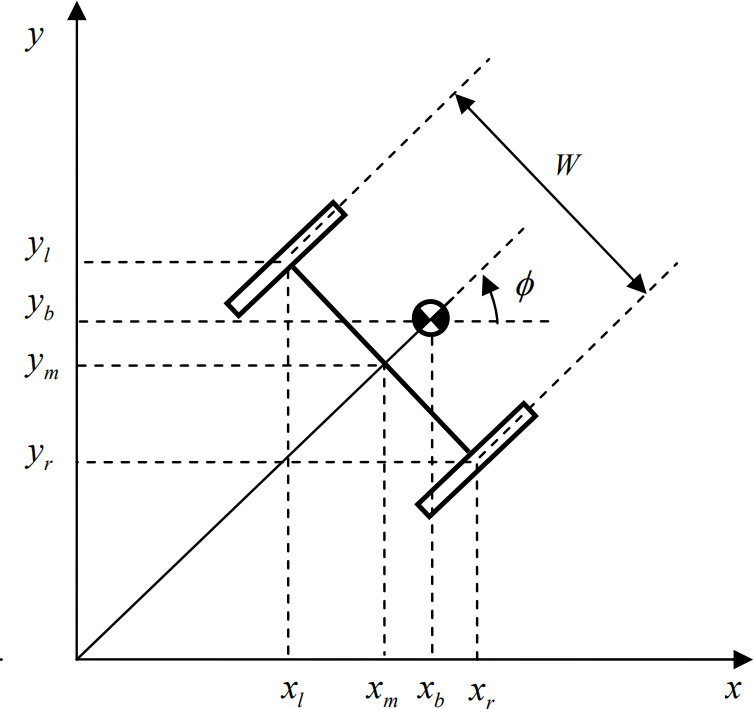
\includegraphics[width=\linewidth]{segway_shora.png}}
    \caption{Nákres segwaye shora, zapůjčeno z \cite{model_based_design}}
    \label{fig:segway_shora}        
\end{figure}

\begin{figure}[htbp]
    \centerline{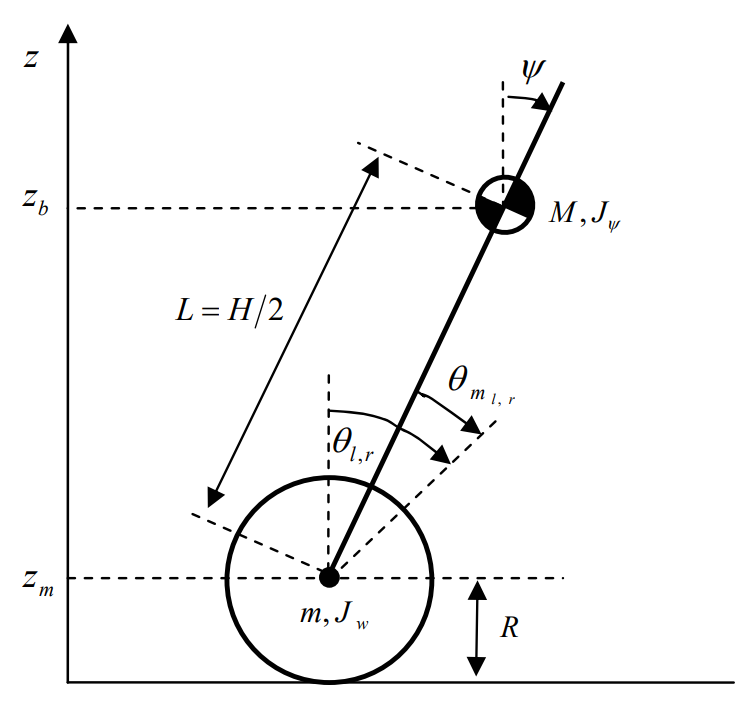
\includegraphics[width=\linewidth]{segway_bok.png}}
    \caption{Nákres segwaye z boku, zapůjčeno z \cite{model_based_design}}
    \label{fig:segway_bok}        
\end{figure}

\section{Matematický model}
Na obrázcích \ref{fig:segway_bok} a \ref{fig:segway_shora} je zaveden souřadný systém a vyznačen význam dalších veličin
nezbytných pro matematický popis segwaye. Odvození matematického modelu je založeno na \cite{model_based_design}.
Uvažujeme tři zobecněné souřadnice
\begin{equation*}
    \begin{split}
        \frac{\theta_l + \theta_r}{2} = \theta~ [\si{rad}] &\cdots \text{Průměrný úhel levého a pravého kola} \\
        \psi ~[\si{rad}] &\cdots \text{Náklon segwaye (osa otáčení v ose koleček)} \\
        \varPhi~[\si{rad}] &\cdots \text{Azimut segwaye (osa otáčení ve svislém směru).}
    \end{split}
\end{equation*}

Tabulka \ref{tab:konstanty} shrnuje všechny konstantní parametry použité při modelování systému včetně jejich hodnot.

\begin{table}[htbp]
    \centering
    \begin{tabular}[t]{|c|c|c|}
        \hline
        symbol & valikost & veličina \\\hline
        $ g $ & 9.81 \si{m/s} & Gravitační zrychlení \\\hline
        $ m $ & 0.03 \si{kg} & Hmotnost kolečka \\\hline
        $ R $ & 0.04 \si{m }& Poloměr kolečka \\\hline
        $ J_w $ & $\frac{mR^2}{2}$ \si{kg . m^2} & Moment setrvačnosti kolečka \\\hline
        $ M $ & 0.6   \si{kg} & Hmotnost segwaye \\\hline
        $ W $ & 0.14  \si{ m} & Šířka segwaye (délka ve směru osy rotace kol) \\\hline
        $ D $ & 0.04  \si{ m} & Tloušťka segwaye (délka ve směru pohybu) \\\hline
        $ H $ & 0.144 \si{m }& Výška  segwaye \\\hline
        $ L $ & $\frac{H}{2}$ \si{m} & Vzdálenost těžiště segwaye od osy kol \\\hline
        $ J_\psi $ & $\frac{ML^2}{3}$ \si{kg . m^2} & Moment setrvačnosti náklonu segwaye\\\hline
        $ J_\varPhi $ & $\frac{M(W^2 + D^2)}{12}$ \si{kg . m^2} & Moment setrvačnosti rotace segwaye \\\hline
        $ J_m $ & $10^{-5}$ \si{kg . m^2} & Moment setrvačnosti motoru \\\hline
        $ R_m $ & 6.69 $\Omega$ & Odpor motoru \\\hline
        $ K_b $ & 0.468 \si{V.s/rad} & EMF kontanta motoru \\\hline
        $ K_t $ & 0.317 \si{Nm/A} & Konstanta kroutivého momentu motoru \\\hline
        $ n $ & 1 [-] & Převodní poměr převodovky \\\hline
        $ f_m $ & 0.0022 [-] & Koeficient tření mezi motorem a segwayem \\\hline
        $ f_w $ & 0 [-] & Koeficient tření mezi kolem a podložkou \\\hline
        
    \end{tabular}
    \caption{Konstantní parametry modelu segwaye}
    \label{tab:konstanty}
\end{table}

\subsection{Nelineární rovnice}
Pomocí analýzy geometrie úlohy lze určit Lagrangián a jeho derivováním podle zobecnělých souřadnic 
následně pro soustavu sestavit obecné pohybové rovnice \eqref{eq:pohyb1}, \eqref{eq:pohyb2} a \eqref{eq:pohyb3}.

\begin{equation}
    \begin{aligned}
        &\left[(2m + M) R^2 + 2 J_w + 2n^2 J_m\right] \ddot{\theta} + \\
        &+ (MLR \text{cos} \psi - 2n^2 J_m) \ddot{\psi} - MLR\dot{\psi}^2 \text{sin} \psi = F_\theta,
    \end{aligned}
    \label{eq:pohyb1}
\end{equation}
\begin{equation}
    \begin{aligned}
        & (MLR \text{cos} \psi - 2n^2 J_m) \ddot{\theta} + (ML^2 + J_\psi + 2n^2 J_m) \ddot{\psi} - \\
        & - MgL\text{sin}\psi - ML^2\dot{\varPhi}^2 \text{sin} \psi \text{cos} \psi = F_\psi,
    \end{aligned}
    \label{eq:pohyb2}
\end{equation}
\begin{equation}
    \begin{aligned}
        &\left[ \frac{1}{2} mW^2  + J_\varPhi + \frac{W^2}{2R^2}\left( J_w + n^2 J_m \right) + ML^2 \text{sin}^2 \psi \right] \ddot{\varPhi} + \\
        &+ 2ML^2 \dot{\psi} \dot{\varPhi} \text{sin}\psi \text{cos} \psi = F_\varPhi.
    \end{aligned}
    \label{eq:pohyb3}
\end{equation}

Zobecněné síly na pravé straně rovnic lze vyjádřit jako
\begin{equation}
    F_\theta = \alpha(v_l + v_r) - 2(\beta + f_w) \dot{\theta} + 2\beta\dot{\psi}
    \label{eq:motor1}
\end{equation}
\begin{equation}
    F_\psi = -\alpha(v_l + v_r) + 2\beta \dot{\theta} - 2\beta \dot{\psi}
    \label{eq:motor2}
\end{equation}
\begin{equation}
    F_\varPhi = \frac{W}{2R} \alpha (v_l - v_r) - \frac{W^2}{2R^2}(\beta + f_w) \dot{\varPhi}
    \label{eq:motor3}
\end{equation}
kde symboly $\alpha$ a $\beta$ jsou substitucemi za následující výrazy
\begin{equation}
    \begin{split}
        \alpha &= \frac{n \cdot K_t} {R_m}  \\
        \beta &= \frac{n \cdot K_t \cdot K_b} {R_m} + f_m 
    \end{split}
    \label{eq:motor_substituce}
\end{equation}

\subsection{Základní úpravy modelu}
S ohledem na charakter úlohy popsané v sekci \ref{sec:uvod} si lze dovolit dvě základní zjednodušení. Protože segway
má pouze balancovat nebo jezdit po rovné čáře, bude jeho azimut $\varPhi$ vždy konstantní. 
Bez újmy na obecnosti lze postavit dokonce $\varPhi = 0$ (odtud i $\dot{\varPhi} = \ddot{\varPhi} = 0$),
čímž se z modelu úplně eliminuje rovnice \eqref{eq:pohyb3}
a rovnice \eqref{eq:pohyb2} se zjednoduší vynulováním jednoho sčítance. Zároveň již není potřeba pracovat se silou $F_\varPhi$
a rovnice \eqref{eq:motor3} tak též může být odstraněna.

Další zjednodušní plyne z rozhodnutí řídit levý i pravý motor stejným napětím $v_l = v_r = v$.
Toto zjednodušení má vliv na rovnice \eqref{eq:motor1} a \eqref{eq:motor2}.

Protože je cílem řízení robota po rovné čáře, je nezbytné udržovat informaci o uražené vzdálenosti $d(t)$.
Protože platí vztah 
\begin{equation}
    d(t) = \int_{-\infty}^t v(t) \text{d}t = \int_ {-\infty}^t \dot{\theta}(t) R \text{d}t = R \theta(t),
    \label{eq:vzdalenost}
\end{equation}
není nezbytné přidávat vzdálenost $d$ jako další stav robota, neboť je lineární funkcí již existujícícho stavu $\theta$.

Nová sada rovnic popisujících systém má tvar
\begin{equation}
    \begin{aligned}
        &\left[(2m + M) R^2 + 2 J_w + 2n^2 J_m\right] \ddot{\theta} + \\
        &+ (MLR \text{cos} \psi - 2n^2 J_m) \ddot{\psi} - MLR\dot{\psi}^2 \text{sin} \psi = F_\theta
    \end{aligned}
    \label{eq:pohyb1_easy}
\end{equation}
\begin{equation}
    \begin{aligned}
        & (MLR \text{cos} \psi - 2n^2 J_m) \ddot{\theta} + \\
        & + (ML^2 + J_\psi + 2n^2 J_m) \ddot{\psi} - MgL\text{sin}\psi = F_\psi
    \end{aligned}
    \label{eq:pohyb2_easy}
\end{equation}

\begin{equation}
    F_\theta = 2v \alpha - 2(\beta + f_w) \dot{\theta} + 2\beta\dot{\psi}
    \label{eq:motor1_easy}
\end{equation}
\begin{equation}
    F_\psi = - 2v \alpha + 2\beta \dot{\theta} - 2\beta \dot{\psi}
    \label{eq:motor2_easy}
\end{equation}

\subsection{Linearizace}
\label{sec:linearizace}

Základním cílem úlohy je stabilizace robota ve svislé poloze, což je zvolený pracovní bod.
Platí pro něj $\psi_p = 0$. Na konkrétní úhel natočení koleček $\theta_p$ není třeba klást žádný požadavek,
protože úloha je translačně invariantní a fyzika segwaye nezávisí na tom, jakou vzdálenost již urazil.
Bez újmy na obecnosti lze zvolit $\theta_p = 0$, protože se tento stav stejně v žádné rovnici přímo nevyskytuje.

V okolí pracovního bodu lze provést aproximaci $\text{cos}(\psi) \approx 1$, $\text{sin}(\psi) \approx \psi$. Rovněž výraz $\dot{\psi}^2$ se bude limitně blížit nule,
protože pro stabilní systém není žádoucí velká úhlová rychlost. Rovnice \eqref{eq:pohyb1_easy} a \eqref{eq:pohyb2_easy} se zjednoduší na
\begin{equation}
    \left[(2m + M) R^2 + 2 J_w + 2n^2 J_m\right] \ddot{\theta} + (MLR - 2n^2 J_m) \ddot{\psi} = F_\theta
    \label{eq:pohyb1_lin}
\end{equation}
\begin{equation}
    (MLR - 2n^2 J_m) \ddot{\theta} + (ML^2 + J_\psi + 2n^2 J_m) \ddot{\psi} - MgL \psi = F_\psi
    \label{eq:pohyb2_lin}
\end{equation}

Pro zjednodušení rovnic \eqref{eq:pohyb1_lin}, \eqref{eq:pohyb2_lin}, \eqref{eq:motor1_easy} a \eqref{eq:motor2_easy}
je možné sdružit konstantní koeficienty do nových 
\begin{equation}
    \begin{split}
        k_1 &= (2m + M) R^2 + 2 J_w + 2n^2 J_m \\
        k_2 &= MLR - 2n^2 J_m \\
        k_3 &= ML^2 + J_\psi + 2n^2 J_m \\
        k_4 &= MgL \\
        c_1 &= 2(\beta + f_w),
    \end{split}
\end{equation}
s tímto označením mají linearizované rovnice tvar
\begin{equation}
    k_1 \ddot{\theta} + k_2 \ddot{\psi} = 2v \alpha - c_1 \dot{\theta} + 2\beta\dot{\psi}
    \label{eq:pohyb1_lin_simple}
\end{equation}
\begin{equation}
    k_2 \ddot{\theta} + k_3 \ddot{\psi} - k_4 \psi = - 2v \alpha + 2\beta \dot{\theta} - 2\beta \dot{\psi}.
    \label{eq:pohyb2_lin_simple}
\end{equation}

Pro získání stavových rovnic je nezbytné osamostatnit z \eqref{eq:pohyb1_lin_simple} a \eqref{eq:pohyb2_lin_simple}
druhé derivace veličin $\theta$ a $\psi$. Analytické řešení vede na vztahy
\begin{equation}
    \begin{split}
        \ddot{\theta} & = \frac{2\beta (k_2 + k_3) \dot{\psi}  - (2 \beta k_2 + c_1 k_3) \dot{\theta} - k_2 k_4 \psi + 2 \alpha (k_2 + k_3) v}{k_1 k_3 - k_2^2} \\
        \ddot{\psi} &= \frac{- 2 \beta (k_1 + k_2) \dot{\psi} + (2 \beta k_1 + c_1 k_2)\dot{\theta}  + k_1 k_4 \psi - 2 \alpha (k_1 + k_2) v}{k_1 k_3 - k_2^2},
        \label{eq:druhe_derivace}
    \end{split}
\end{equation}
které lze dále zjednodušit sdružením kostantních parametrů. Označením
\begin{equation*}
    a_1 = \frac{2\beta (k_2 + k_3)}{k_1 k_3 - k_2^2}, \\
\end{equation*}
\begin{equation*}
    a_2 = -\frac{2 \beta k_2 + c_1 k_3}{k_1 k_3 - k_2^2}, \\
\end{equation*}
\begin{equation*}
    a_3 = -\frac{k_2 k_4}{k_1 k_3 - k_2^2}, \\
\end{equation*}
\begin{equation*}
    a_4 = \frac{2 \alpha (k_2 + k_3)}{k_1 k_3 - k_2^2}, \\
\end{equation*}
\begin{equation*}
    a_5 = -\frac{2 \beta (k_1 + k_2)}{k_1 k_3 - k_2^2}, \\
\end{equation*}
\begin{equation*}
    a_6 = \frac{2 \beta k_1 + c_1 k_2}{k_1 k_3 - k_2^2}, \\
\end{equation*}
\begin{equation*}
    a_7 = \frac{ k_1 k_4 }{k_1 k_3 - k_2^2}, \\
\end{equation*}
\begin{equation*}
    a_8 = -\frac{2 \alpha (k_1 + k_2)}{k_1 k_3 - k_2^2}, \\
\end{equation*}
se rovnice \eqref{eq:druhe_derivace} zjednoduší na
\begin{equation}
    \begin{split}
        \ddot{\theta} & = a_1 \dot{\psi} + a_2  \dot{\theta} + a_3  \psi + a_4  v, \\
        \ddot{\psi} &= a_5  \dot{\psi} + a_6  \dot {\theta} + a_7  \psi + a_8  v.
        \label{eq:druhe_derivace_easy}
    \end{split}
\end{equation}

Přeznačme fyzikální veličiny v rovnici \eqref{eq:druhe_derivace_easy} podle konvence v oboru automatického řízení.
Zaveďme $u(t) = v(t)$ pro vstup systému a $\vec{x}$ pro vektor stavů systému
\begin{equation}
    \vec{x} = \begin{bmatrix}
        x_1 \\
        x_2 \\
        x_3 \\
        x_4
    \end{bmatrix} = \begin{bmatrix}
        \theta \\
        \psi \\
        \dot{\theta} \\
        \dot{\psi}
    \end{bmatrix}.
\end{equation}
Přeznačením výrazů v rovnici \eqref{eq:druhe_derivace_easy} vznikají stavové rovnice pro stavy $x_3$ a $x_4$. 
Spolu s triviálními rovnicemi pro stavy $x_1$ a $x_2$ vzniká kompletní systém stavových rovnic systému
\begin{equation}
    \begin{split}
        \dot{x_1} &= x_3 \\
        \dot{x_2} &= x_4 \\
        \dot{x_3} & = a_1 x_4 + a_2 x_3 + a_3 x_2 + a_4 u \\
        \dot{x_4} &= a_5  x_4 + a_6 x_3 + a_7 x_2 + a_8 u,
        \label{eq:stavove_rovnice}
    \end{split}
\end{equation}
jejž lze převést do maticové podoby
\begin{equation}
    \dot{\vec{x}} = \mathbf{A} \Delta \vec{x} + \mathbf{B} \Delta u, \\
\end{equation}
kde matice systému a matice vstupní mají tvar
\begin{equation}
    \mathbf{A} = \begin{bmatrix}
        0 & 0 & 1 & 0 \\
        0 & 0 & 0 & 1 \\
        0 & a_3 & a_2 & a_1 \\
        0 & a_7 & a_6 & a_5
    \end{bmatrix} ~~~~ \mathbf{B} = \begin{bmatrix}
        0 \\ 0 \\a_4 \\a_8
    \end{bmatrix}
\end{equation}

\subsection{Vyčíslení v pracovním bodě}

Pracovní bod zvolený již v sekci \ref{sec:linearizace} odpovídá nestabilnímu ekvilibriu ve svislé pozici segwaye.
Ve stavovém prostoru přísluší tomuto rovnovážnému bodu vektor 
\begin{equation}
    P = \begin{bmatrix}
        \theta_p &    \psi_p &     \dot{\theta}_p &     \dot{\psi}_p & u_p
    \end{bmatrix} = \begin{bmatrix}
        0 & 0 & 0 & 0 & 0
    \end{bmatrix}.
\end{equation}
Pomocí hodnot konstant uvedených v tabulce \ref{tab:konstanty} je možné vyčíslit prvky matic $\mathbf{A}$ a $\mathbf{B}$ stavového modelu. Platí
\begin{equation}
        \mathbf{A} = \begin{bmatrix}
            0 & 0 & 1 & 0 \\
            0 & 0 & 0 & 1 \\
            0 & -409.7184 & -162.1273 & 162.1273 \\
            0 & 269.6273 & 78.1496 & -78.1496
        \end{bmatrix}
    \end{equation}
    \begin{equation}
        \mathbf{B} = \begin{bmatrix}
            0 \\ 0 \\ 315.1597 \\ -151.9152
        \end{bmatrix}.
    \end{equation}
Tím je nalezena lineární náhrada obecně nelineárního systému v okolí pracovního bodu a modelování systému je hotovo.



\begin{thebibliography}{9}

    \bibitem{model_based_design}
    Yorihisa Yamamoto, \emph{NXTway-GS Model-Based Design} 
    \end{thebibliography}

\end{document}
